\section{Autres contributions à \cite{koung_consensus-based_2020}}

\subsection{Calculs des points cibles}

Pour piloter l'essaim, un unique point cible global est envoyé à l'ensemble des robots de l'essaim. Cependant, chaque robot ne cherche pas à atteindre ce point directement. Au lieu de cela, chacun calcule son propre point cible individuel en réalisant la translation du point-cible globale par un \textbf{vecteur relatif} correspondant à sa position initiale par rapport au barycentre de l'essaim. Formellement, pour le robot $i$, le point cible individuel $\mathbf{p}_r^i$ est donné par :
\begin{equation}
\mathbf{p}_r^i = \mathbf{p}_\text{goal} + (\mathbf{p}_i^\text{init} - \mathbf{p}_\text{bary}^\text{init})
\end{equation}
où $\mathbf{p}_\text{goal}$ est la cible globale, $\mathbf{p}_i^\text{init}$ la position initiale du robot $i$, et $\mathbf{p}_\text{bary}^\text{init}$ le barycentre initial de l'essaim.

L'intérêt de cette approche est de préserver la formation relative des robots à l'arrivée l'essaim. Ainsi, même si tous les robots reçoivent la même consigne globale, chacun vise une position différente qui maintient la structure de l'essaim autour du barycentre. 

\begin{figure}[h!]
    \centering
    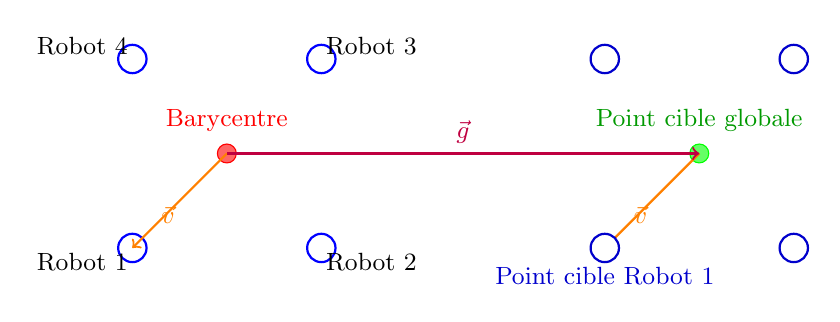
\begin{tikzpicture}[scale=1.2]
        % Robots (carré, cercles blancs)
        \filldraw[fill=white,draw=blue,thick] (0,0) circle (0.15) node[below left=-2pt] {\small Robot 1};
        \filldraw[fill=white,draw=blue,thick] (2,0) circle (0.15) node[below right=-2pt] {\small Robot 2};
        \filldraw[fill=white,draw=blue,thick] (2,2) circle (0.15) node[above right=-2pt] {\small Robot 3};
        \filldraw[fill=white,draw=blue,thick] (0,2) circle (0.15) node[above left=-2pt] {\small Robot 4};
        % Barycentre
        \filldraw[fill=red!60,draw=red] (1,1) circle (0.10);
        \node[red] at (1,1.35) {\small Barycentre};
        % Vecteur relatif pour Robot 1
        \draw[->,thick,orange] (1,1) -- (0,0) node[midway,below left=-2pt,orange] {\small $\vec{v}$};
        % Point cible global (plus loin à droite)
        \filldraw[fill=green!60,draw=green] (6,1) circle (0.10);
        \node[green!60!black] at (6,1.35) {\small Point cible globale};
        % Vecteur relatif reporté (même style que le vecteur initial)
        \draw[->,thick,orange] (6,1) -- (5,0) node[midway,below left=-2pt,orange] {\small $\vec{v}$};
        % Nouveau point cible individuel pour Robot 1
        \filldraw[fill=white,draw=blue!80!black,thick] (5,0) circle (0.15);
        \node[blue!80!black] at (5,-0.3) {\small Point cible Robot 1};
        % Vecteur barycentre -> point cible globale
        \draw[->,thick,purple] (1,1) -- (6,1) node[midway,above,sloped,purple] {\small $\vec{g}$};
        % Autres points cibles individuels
        \filldraw[fill=white,draw=blue!80!black,thick] (7,0) circle (0.15);
        \filldraw[fill=white,draw=blue!80!black,thick] (7,2) circle (0.15);
        \filldraw[fill=white,draw=blue!80!black,thick] (5,2) circle (0.15);
    \end{tikzpicture}
    \caption{Illustration du calcul du point cible individuel à partir du barycentre et du vecteur relatif initial. }
    \label{fig:relative_vector_target}
\end{figure}

La Figure \ref{fig:relative_vector_target} ci-dessus illustre la méthode. Le vecteur relatif $\vec{v}$ permet de déterminer la cible individuelle du robot. Le vecteur $\vec{g}$ relie le barycentre au point cible global et symbolise le déplacement global de l'essaim.

%----------------------------------------------------------------------------
%----------------------------------------------------------------------------

\subsection{Adaptation du coefficient $c_{1}^{\gamma}$}

Le coefficient $c_{1}^{\gamma}$ détermine la force avec laquelle chaque robot est attiré vers son point cible. Formellement, il intervient dans le terme de contrôle suivant :
\begin{equation}
\mathbf{u}_\gamma = -c_{1}^{\gamma} (\mathbf{p}_i - \mathbf{p}_r)
\end{equation}
où $\mathbf{p}_i$ est la position du robot $i$ et $\mathbf{p}_r$ la position de référence.

Un $c_{1}^{\gamma}$ élevé permet à l'essaim de converger rapidement vers la cible. Cependant, en présence de perturbations (par exemple, un robot décalé ou une erreur de formation), maintenir une attraction vers le point cible peut aggraver la situation : les robots continueraient à avancer vers la cible sans corriger la formation car le terme $u_{i}^{\alpha}$, responsable du maintien de la formation, met un certain temps à converger. 
Pour éviter cela, l'idée est d'adapter dynamiquement $c_{1}^{\gamma}$ : lorsqu'une perturbation est détectée (écart de distance par exemple), $c_{1}^{\gamma}$ est réduit afin de ralentir, voire stopper, le déplacement global de l'essaim. Cela laisse le temps au système de corriger la formation avant de poursuivre la progression vers la cible.


Cette adaptation repose sur la surveillance des ratios de distance et des erreurs d'angle entre robots. Si tous les robots respectent les tolérances, $c_{1}^{\gamma}$ garde sa valeur normale, et l'essaim se déplace normalement. Sinon, il est réduit selon la gravité de la perturbation.

\begin{equation}
r_d = \frac{d_\text{actuelle}}{d_\text{désirée}}; \quad \epsilon_\theta = \min\left(|\theta_\text{actuel} - \theta_\text{cible}|, 2\pi - |\theta_\text{actuel} - \theta_\text{cible}|\right)
\end{equation}
Avec $r_d$ le ratio de distance et $\epsilon_\theta$ l'erreur d'angle.
Le coefficient est alors adapté selon :
\begin{equation}
c_{1}^{\gamma} = c_{1,\text{base}}^{\gamma} \cdot f_d \cdot f_\theta
\end{equation}
où $f_d$ et $f_\theta$ sont des facteurs de réduction dépendant respectivement des écarts de distance et d'angle, calculés par exemple comme :
\begin{equation}
f_d = e^{-k_d \cdot \delta_d}
\end{equation}
\begin{equation}
f_\theta = e^{-k_\theta \cdot \delta_\theta}
\end{equation}
avec $\delta_d$ et $\delta_\theta$ les déviations normalisées, et $k_d$, $k_\theta$ des constantes d'ajustement.
Une adaptation exponentielle a été choisie, afin de réduire rapidement $c_{1}^{\gamma}$ en cas de perturbation, permettant par exemple de stopper le déplacement de l'essaim si un robot se dirige droit vers un autre, évitant ainsi la collision.

Les valeurs des paramètres $k_d$, $k_\theta$, $\delta_d$ et $\delta_\theta$ ont été déterminées expérimentalement. Le tableau ci-dessous résume les valeurs utilisées :

\begin{table}[h!]
    \centering
    \begin{tabular}{|c|c|c|c|c|}
        \hline
         $k_d$ & $k_\theta$ & $\delta_d$ (seuil) & $\delta_\theta$ (seuil) \\
        \hline
          0.4 & 0.2 & 0.10 & 0.08 \\
        \hline
    \end{tabular}
    \caption{Valeurs expérimentales des paramètres d'adaptation de $c_{1}^{\gamma}$}
\end{table}

Ces seuils correspondent à des tolérances relatives sur les distances et les angles (par exemple, $\delta_d = 0.10$ signifie une tolérance de $\pm10\%$ sur la distance désirée).

Pour éviter des variations trop brusques de $c_{1}^{\gamma}$ (qui pourraient entraîner des mouvements saccadés ou instables), un lissage exponentiel est appliqué à chaque itération :
\begin{equation}
c_{1}^{\gamma}(t) = \alpha \cdot c_{1}^{\gamma}(t-1) + (1-\alpha) \cdot c_{1}^{\gamma_{\text{calculé}}}
\end{equation}
où $\alpha$ est le facteur de lissage (typiquement $\alpha = 0.9$).

Chaque robot calcule donc indépendamment sa propre valeur de $c_{1}^{\gamma}$ en fonction de ses mesures locales. Cela n'est pas problématique pour la cohésion de l'essaim : si un robot détecte une perturbation et réduit son $c_{1}^{\gamma}$, il ralentit son déplacement vers le point cible. Les autres robots, via les tolérances sur les distances et les angles, vont également détecter ce ralentissement (car leurs propres ratios vont sortir des seuils) et adapter leur $c_{1}^{\gamma}$ en conséquence. Ainsi, même si les valeurs de $c_{1}^{\gamma}$ diffèrent temporairement, le terme $u_i^\alpha$ (responsable du maintien de la formation) reprend naturellement le dessus et assure la cohésion et la correction de la formation avant la reprise du déplacement global.



